% !TEX program = xelatex
% !TEX encoding = UTF-8  (utf8)

%\documentclass[glossy]{beamer}
\documentclass[glossy,handout]{beamer}

\mode<presentation>{
	\useoutertheme{wuerzburg}
	\useinnertheme[realshadow,corners=2pt,padding=2pt]{chamfered}
	\usecolortheme{shark}
	\usefonttheme{serif}
	\usefonttheme{professionalfonts}
	\usefonttheme{structurebold}
}

%%%%% fontspec
\usepackage{fontspec}
\setmainfont[BoldFont={Georgia Bold},
	ItalicFont={Georgia Italic},
	BoldItalicFont={Georgia Bold Italic}
	]{Georgia}

%%%%% XeCJK
\usepackage[AutoFallBack,AutoFakeBold,AutoFakeSlant,
	PunctStyle=CCT]{xeCJK}
\setCJKmainfont[%BoldFont={Adobe Heiti Std},
	ItalicFont={Adobe Kaiti Std},
%	SlantedFont={Adobe Song Std},
    BoldItalicFont={Weibei SC},
%    BoldSlantedFont={Adobe Fangsong Std}
	]{Adobe Heiti Std}
%\usepackage{xeCJKfntef}		%汉字加点和可断行的下划线
\setCJKmathfont{Cambria Math}

%%%%% math settings
\usepackage{amsmath}		%数学环境,align, align*
\usepackage{amsfonts}		%数学字体,mathbb
\usepackage{amssymb}		%数学公式
%\usepackage{amsthm}			%已包含在amsmath中
%\usepackage{mathrsfs}		%数学花体
\usepackage{extarrows}		%\xlongequal
\usepackage{bm}				%bm

\usepackage{xcolor}

\usepackage{graphics}
\usepackage{graphicx}		%definecolor, colorbox, fcolorbox

\usepackage{ulem}			%各种下划线:uline, uuline, uwave, sout, xout
%\usepackage{enumerate}
%\usepackage{esint}			%any type of integral symbol
% \usepackage{tabularx}
% \usepackage{multirow}
% \usepackage{verbatim}
% \usepackage{listings}
%\usepackage{polynom}		%多项式的竖式带余除法
%\usepackage{overpic}		%允许在图片上写文字
%\usepackage{wrapfig}		%支持插入文字环绕的图片
\usepackage{booktabs}		%粗的表格横线

\usepackage{tcolorbox} 		%各种自定义的盒子
\tcbuselibrary{skins, breakable, theorems}

\usepackage{tikz}
\usetikzlibrary{shapes,arrows,positioning,matrix,chains,backgrounds,fit}
\newcommand<>{\hover}[1]{
	\uncover#2{%
	\begin{tikzpicture}[remember picture,overlay]%
	\draw[fill,opacity=0.4] (current page.south west)
	rectangle (current page.north east);
	\node at (current page.center) {#1};
	\end{tikzpicture}}
}

\title{作业讲评}
\author{YB. Tang}
\institute{NUDT}
%\date{\today}
\date{2018-AU}

\begin{document}

%%%%% my macros
%===============macros====================
\def\ds{\displaystyle}
% \def\fin{\hfill$\Box$}
\def\fin{\hfill{\color{green!50!black}$\blacksquare$}}
\def\bs{\bigskip}
\def\b{\color{blue!80!yellow}}
\def\bb{\bf\color{blue}}
\def\e{\ensuremath{\varepsilon}}

\newcommand{\ba}[1]{\alert{\bf #1}}
\providecommand{\mbb}[1]{\ensuremath{\mathbb{{#1}}}}
\providecommand{\mr}[1]{\ensuremath{\mathrm{{#1}}}}


\newcommand{\limn}{\ensuremath{\lim\limits_{n\to\infty}}}
\newcommand*{\limx}[1]{\ensuremath{\lim\limits_{x\to{#1}}}}
\newcommand*{\limdx}{\ensuremath{\lim\limits_{\Delta x\to 0}}}
\providecommand{\llim}[1]{\ensuremath{\lim\limits_{#1}}}

\newcommand{\sumn}[1][1]{\ensuremath{\sum\limits_{n=#1}^{\infty}}}
\providecommand{\sumk}[1]{\ensuremath{\sum\limits_{k={#1}}^n}}
\providecommand{\suml}{\ensuremath{\sum\limits}}

\newcommand*{\df}[2]{\displaystyle\frac{\,{#1}\,}{\,{#2}\,}}
\newcommand*{\dx}{\Delta x}
\renewcommand{\d}{\mathrm{d}}
\newcommand*{\p}{\ensuremath{\partial}}

\newcommand{\dint}{\ensuremath{\displaystyle\int}}

\newcommand{\ps}[1]{$^{[\mbox{\kaiti\footnotesize 注}]}$
\marginpar{\kaiti\small\color{blue} {注:}#1}}

%define tab of .25 textwidth and can auto strech
%\tab{the word}\tab{another word}\tab{3rd one}
\newlength{\tabcont}
\newcommand{\tab}[1]{%
	\settowidth{\tabcont}{#1}%
	\ifthenelse{\lengthtest{\tabcont < .25\linewidth}}%
	{\makebox[.25\linewidth][l]{#1}\ignorespaces}%
	%{\makebox[.5\linewidth][l]{\color{red} #1}\ignorespaces}%
	{\makebox[.5\linewidth][l]{#1}\ignorespaces}%
}%

%set fontsize with number of points
% \newcommand{\fs}[1]{\fontsize{#1 pt}{5pt}\selectfont}

\newtcolorbox{thx}{colframe=blue!40!black,colback=white,breakable}

\newtcolorbox{ext}{colframe=green!60!black,colback=green!20!white,breakable}

\definecolor{shadecolor}{rgb}{0.9,0.9,0.9}

\renewcommand{\thefigure}{\thechapter.\arabic{figure}}

% !TEX root = ../1-main-SL.tex
% !TEX encoding = UTF-8  (utf8)

\begin{frame}
	\centering
	\bf\Huge\color{purple} 习题1-2讲评\\[1cm]
	\small\color{gray}2018-10-24
\end{frame}

\section{说在前面}

\begin{frame}[t]\frametitle{说在前面}
	\linespread{1.8}
	\Large
    \begin{itemize}
    	\item 如何改错?
    	\begin{enumerate}
    		\item {\it\Large 多留空白...}
    		\item {\it\Large 要还是不要,划清界限...}
    	\end{enumerate}
    	\item 对还是错?
    	\begin{enumerate}
    		\item {\it\Large $\sqrt[3]{n+1}-\sqrt[3]{n}<\sqrt{n+1}-\sqrt{n}$.}
    		\item {\it\Large 要证$\limn(a_{n+1}-a_n)=0$,只需证明}
    		$$\limn\df{a_{n+1}}{a_n}=1.$$
    		\item {\it\Large $\{a_n\}$有界,故可设$\limn a_n=A$.}
    	\end{enumerate}
    \end{itemize}
\end{frame}

\section{参考解答}

\begin{frame}[t]\frametitle{1.用极限的定义证明}
\large
(1)$\limn\df{\sqrt{n^2+a^2}}n=1$;

证:\it 对任意$\e>0$,令$N=\left[\df{a^2}{\e}\right]+1>\df{a^2}{\e}$,
则对任意$n>N$,均有
$$\left|\df{\sqrt{n^2+a^2}}n-1\right|
=\df{a^2}{n(\sqrt{n^2+a^2}+n)}<\df{a^2}n<\df{a^2}N<\e,
$$
由数列极限的定义,即证。\fin
\end{frame}

\begin{frame}[t]\frametitle{1.用极限的定义证明}
\large

(2)$\limn0.\underbrace{99\ldots9}_{n\mbox{\footnotesize 个}}=1.$

证:\it 对任意$\e>0$,令$N=[-\lg\e]+1$,则对任意$n>N$,均有
$$|0.\underbrace{99\ldots9}_{n\mbox{\footnotesize 个}}-1|
=\df1{10^n}<\df1{10^N}
<\df1{10^{-\lg\e}}=\e,$$
由数列极限的定义,即证。\fin
\end{frame}

\begin{frame}[t]\frametitle{1.用极限的定义证明}
\large

(3)$\limn\left(\sqrt[3]{n+1}-\sqrt[3]{n}\right)=0$.
\bs

证:\it 对任意$\e>0$,令$N=\left[1/\e\right]+1$,则对任意$n>N$,有
$$|\sqrt[3]{n+1}-\sqrt[3]{n}|
=\df1{(n+1)^{\frac{2}{3}}+(n+1)^{\frac13}n^{\frac13}+n^{\frac23}}
<\df1n<\df1N<\e.$$
由数列极限的定义,即证。\fin
\end{frame}

\begin{frame}[t]\frametitle{1.用极限的定义证明}
\large

(4)$\limn\df{n^2-n-1}{2n^2+2n-4}=\df12$.
\bs

证:\it 对任意$\e>0$,令$N=$,则对任意$n>N$有
$$\left|\df{n^2-n-1}{2n^2+2n-4}-\df12\right|
=\left|\df{-2n-3}{2n^2+2n-4}\right|<\df1n<\df1N<\df1{\e}.$$
由数列极限的定义,即证。\fin
\end{frame}

\begin{frame}[t]\frametitle{证明极限的性质}
\large
2.数列$\{a_n\}$有界,$\limn b_n=0$,证明:$\limn a_nb_n=0$。
\end{frame}

\begin{frame}{哪里不太对?}
	\centering
	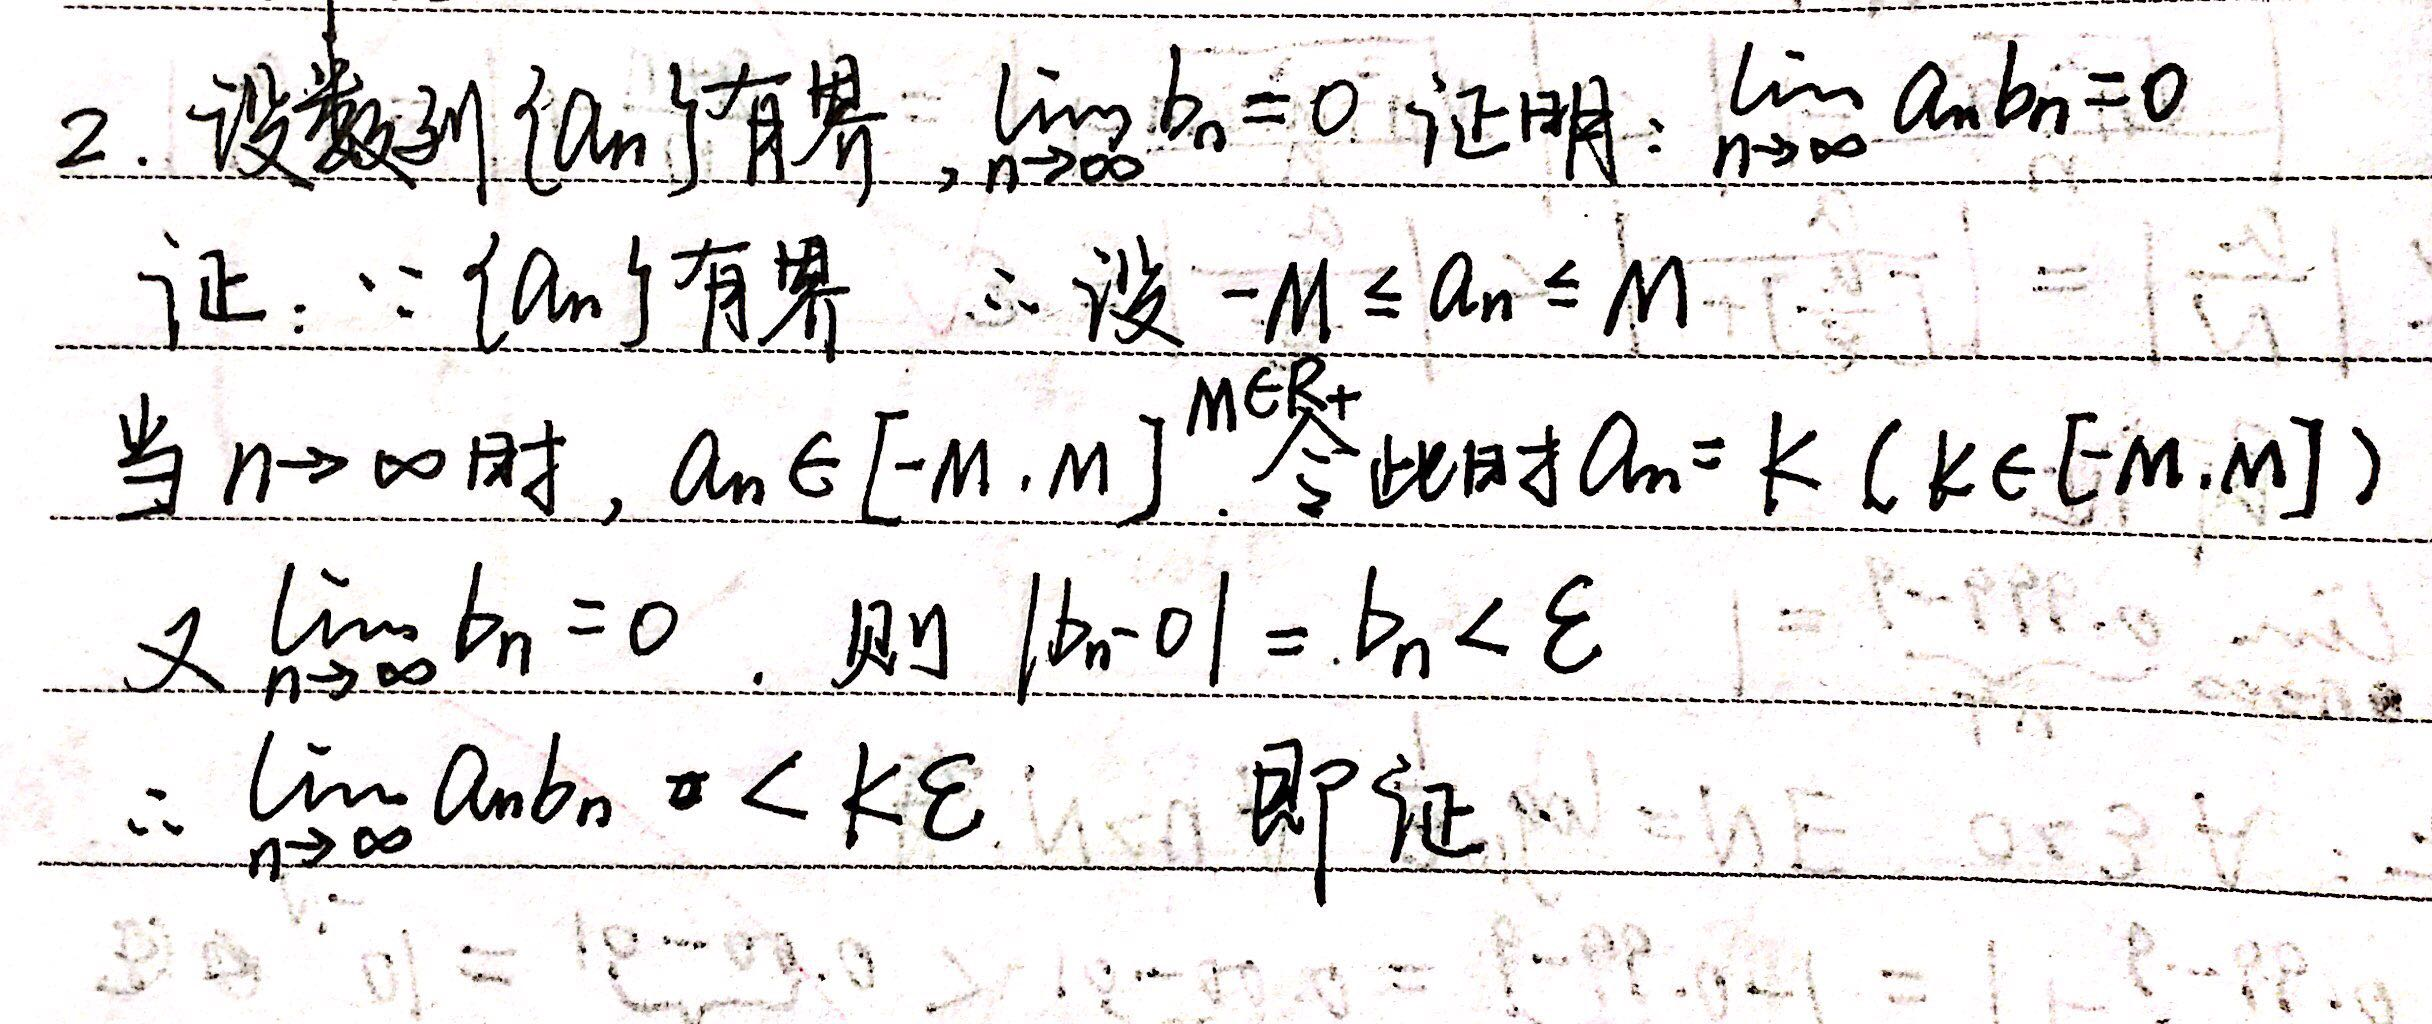
\includegraphics[width=0.9\textwidth]{./images/ch01/HWR/anbn0-1.jpeg}
\end{frame}

\begin{frame}{哪里不太对?}
	\centering
	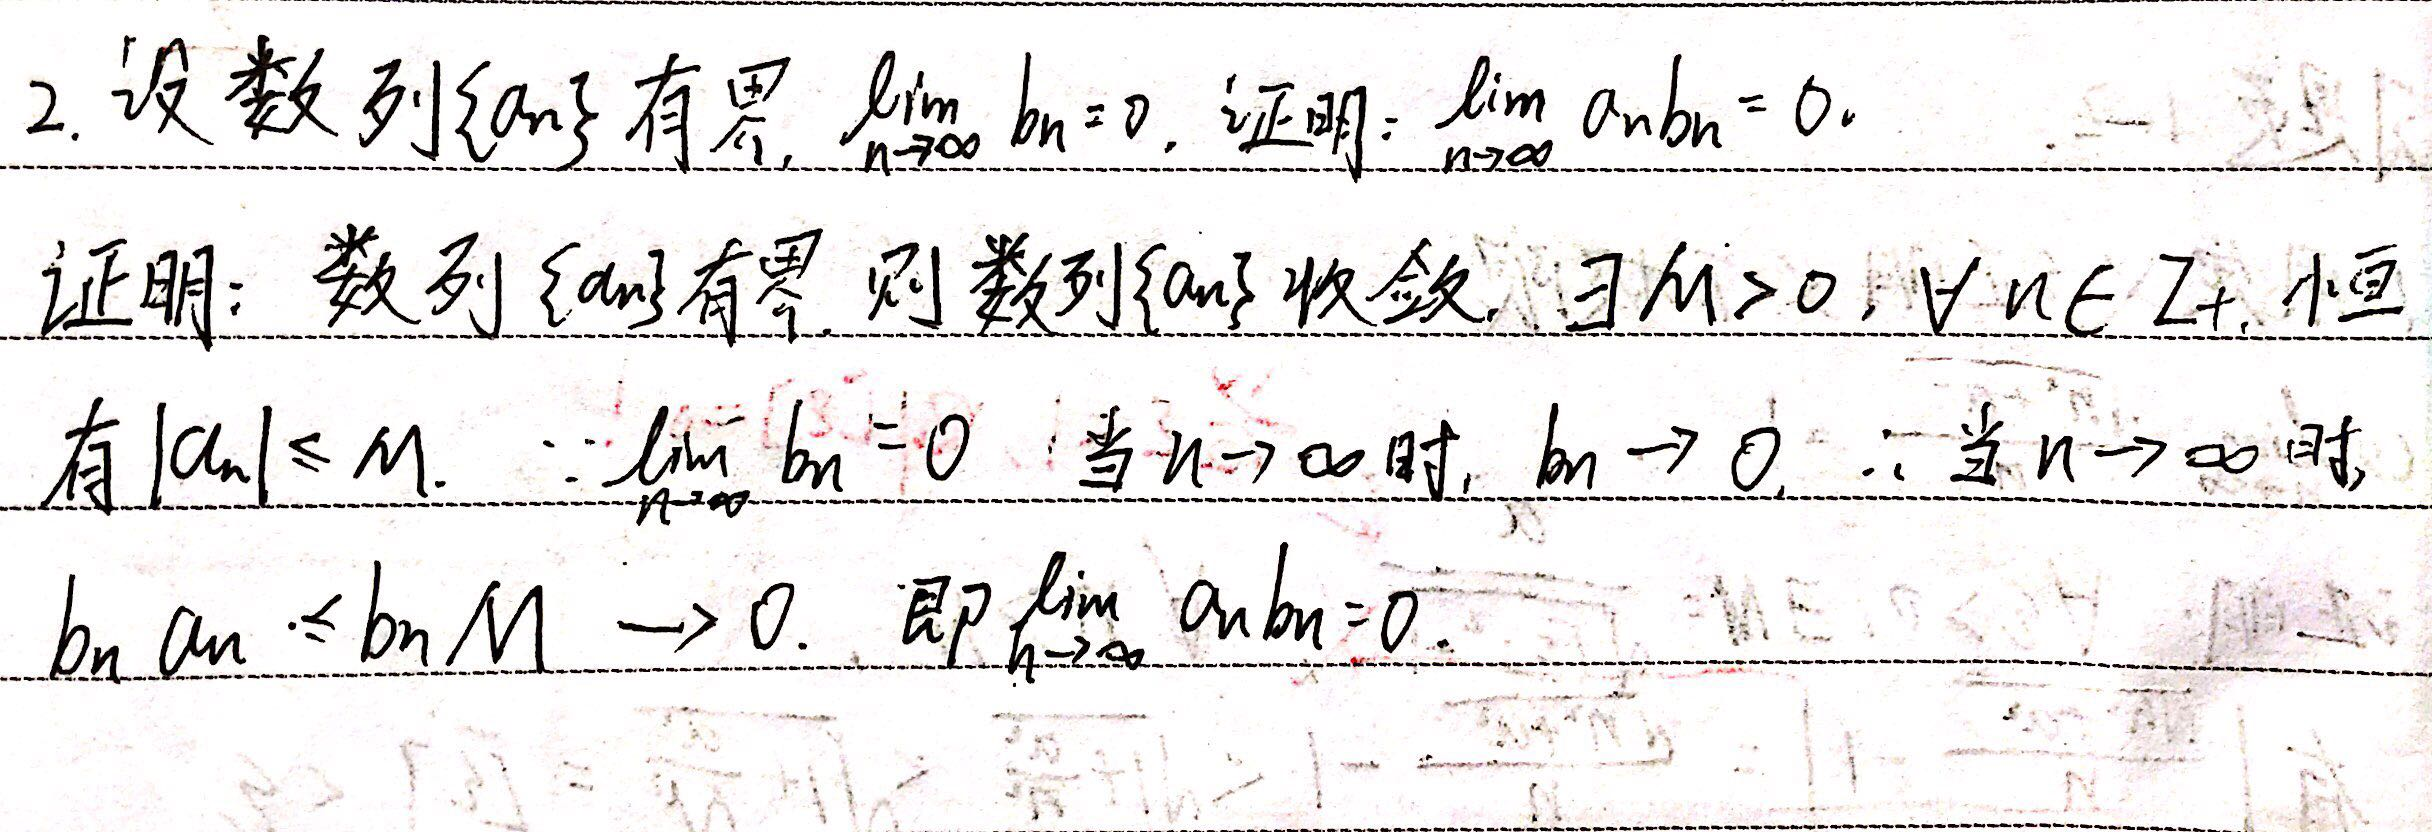
\includegraphics[width=0.9\textwidth]{./images/ch01/HWR/anbn0-2.jpeg}
\end{frame}

\begin{frame}{哪里不太对?}
	\centering
	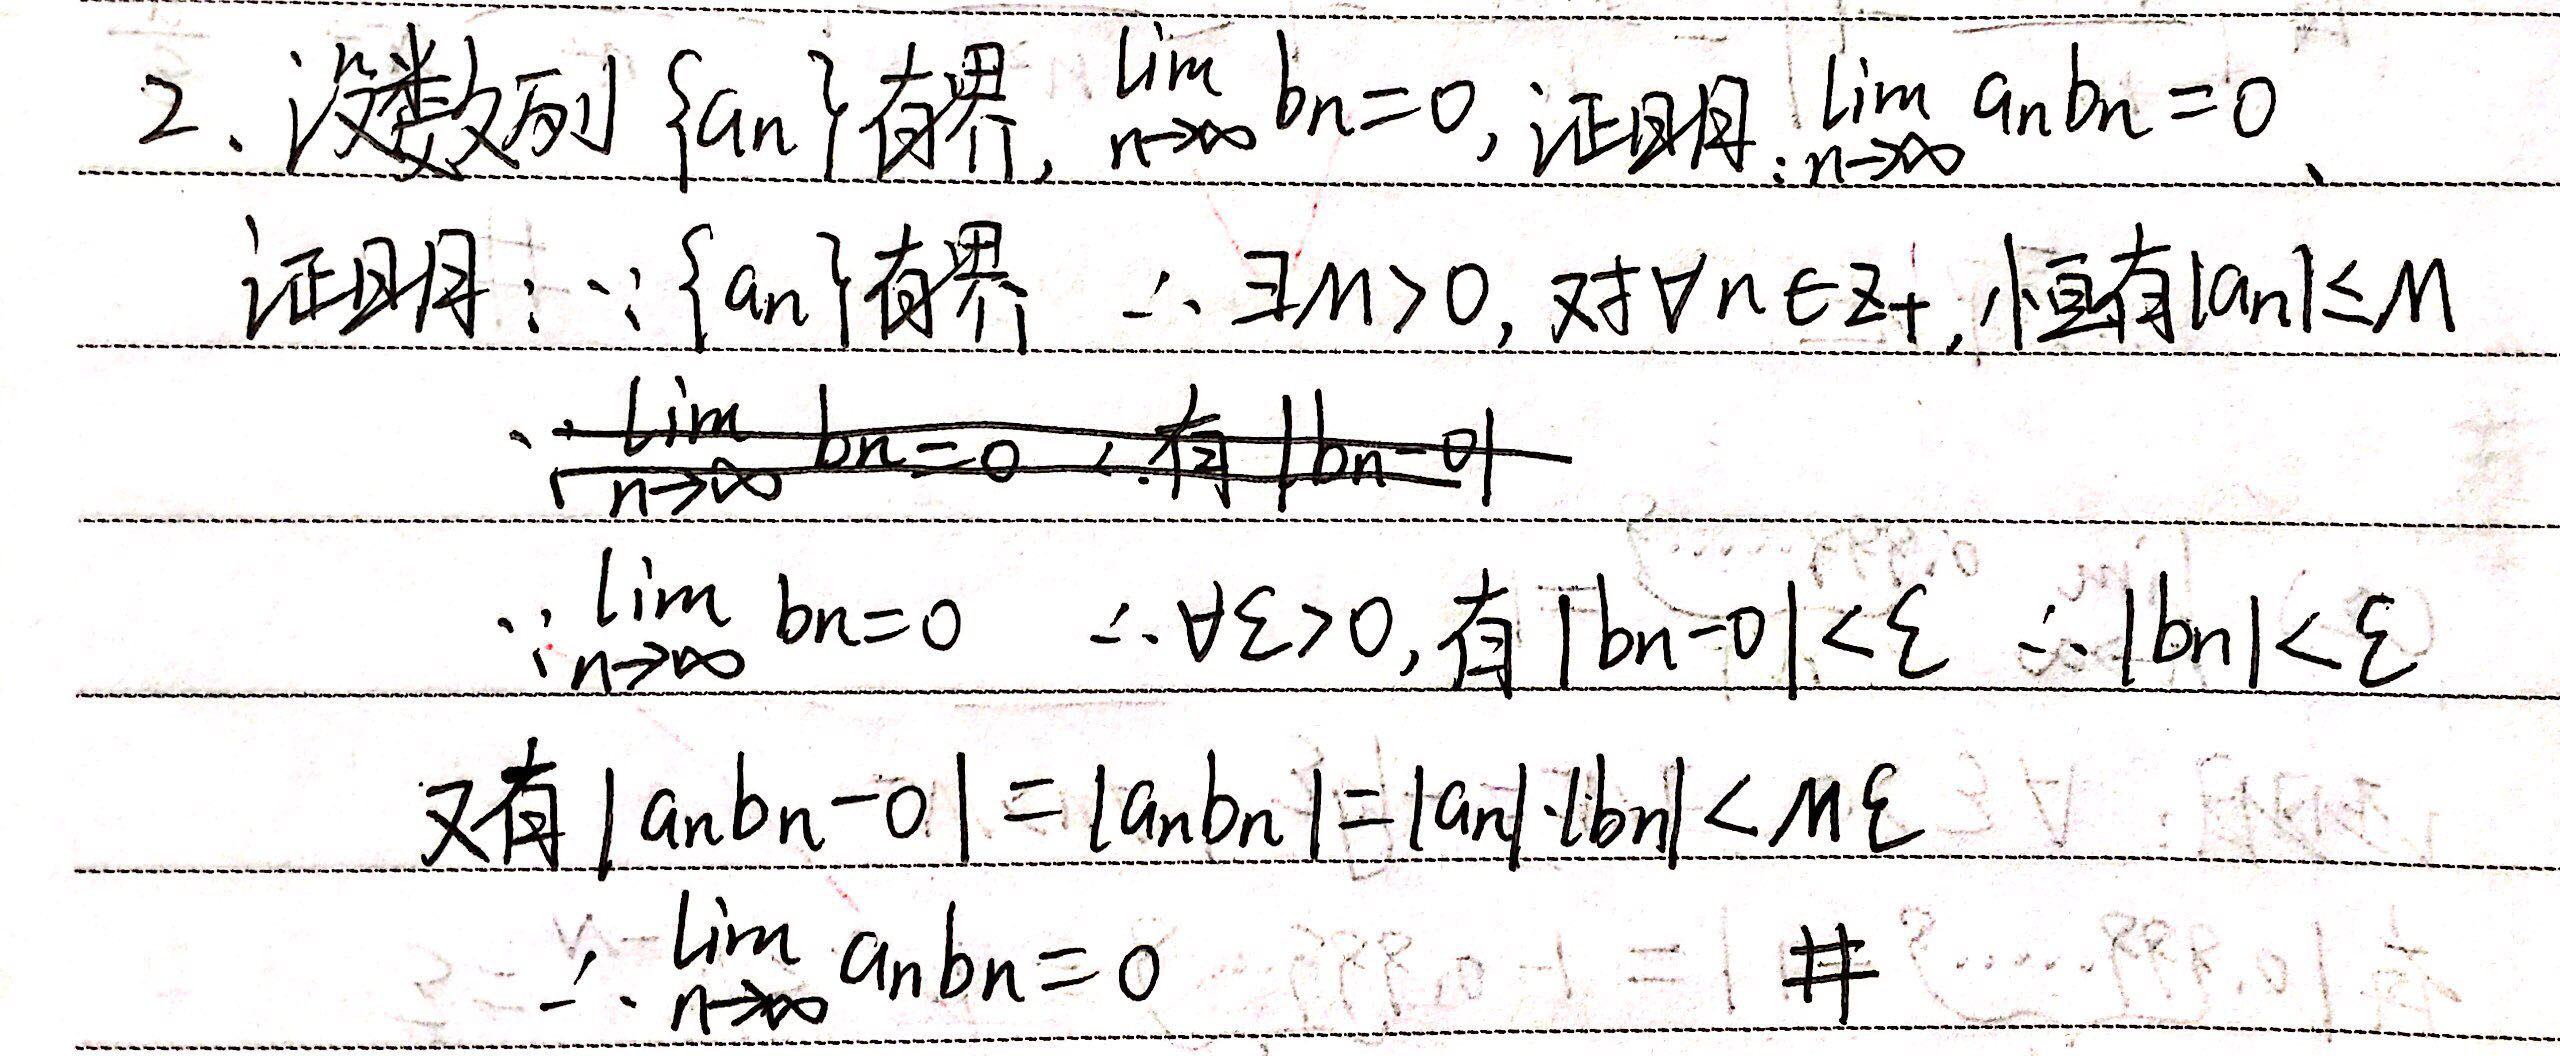
\includegraphics[width=0.9\textwidth]{./images/ch01/HWR/anbn0-3.jpeg}
\end{frame}

\begin{frame}{哪里不太对?}
	\centering
	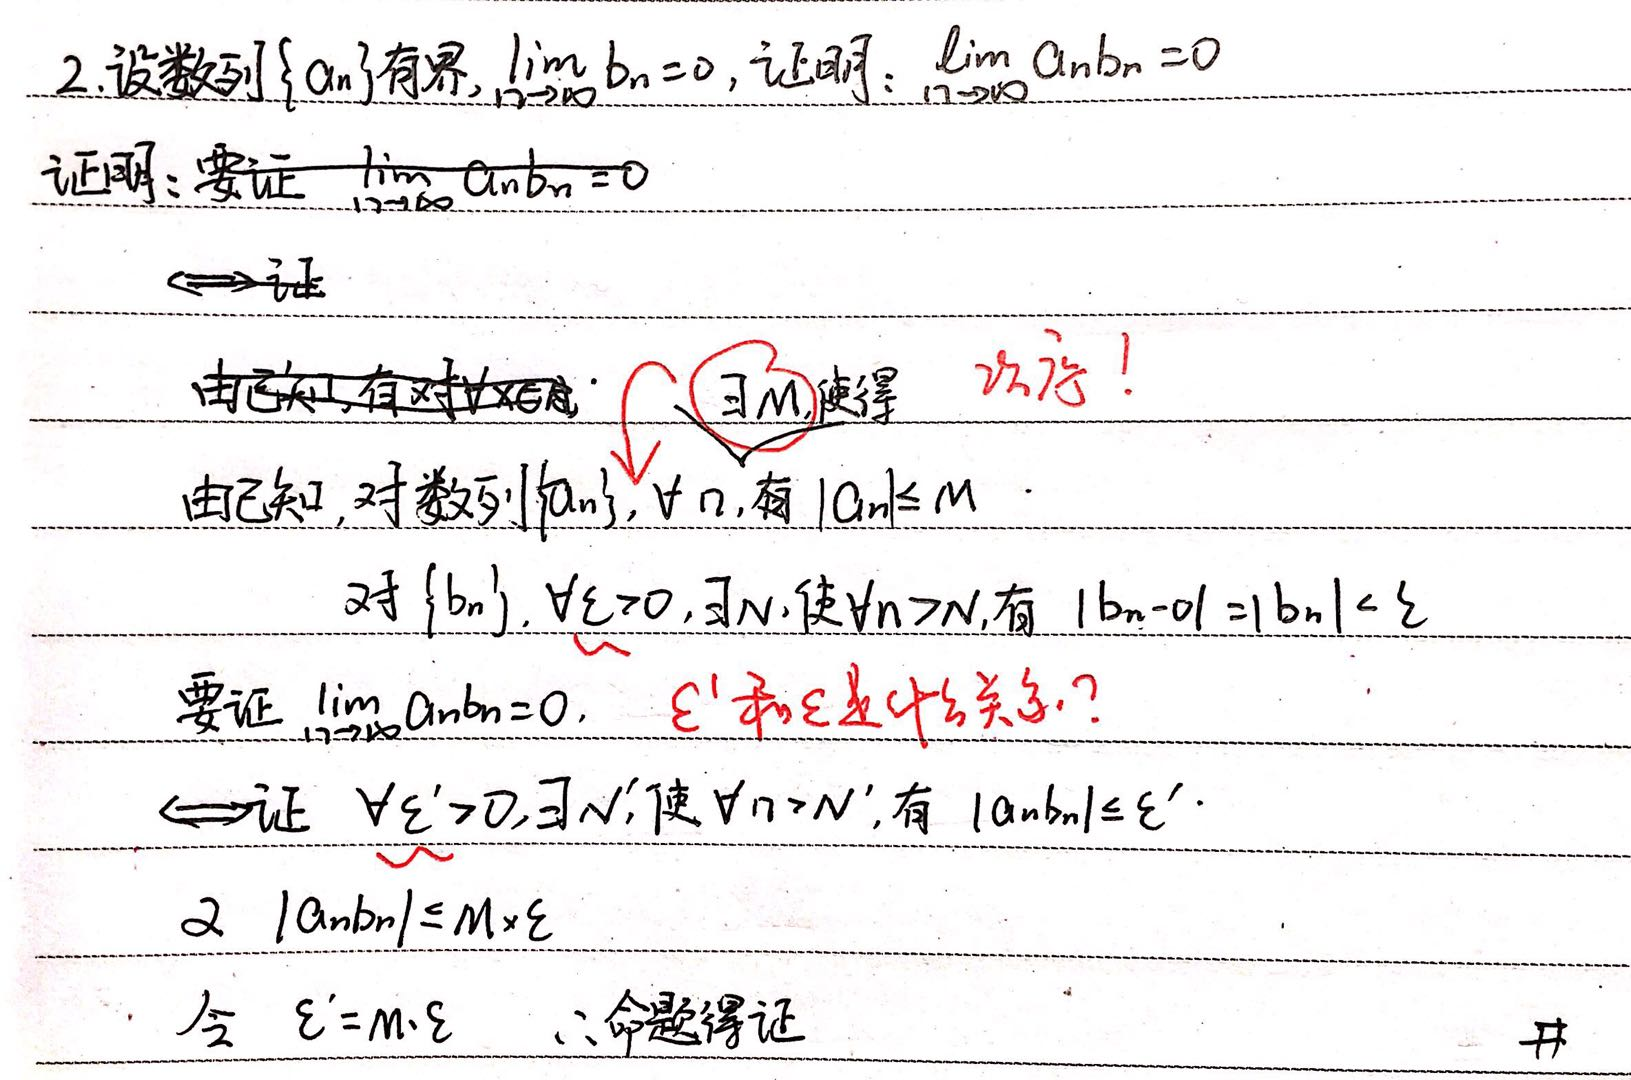
\includegraphics[width=0.9\textwidth]{./images/ch01/HWR/anbn0-4.jpeg}
\end{frame}

\begin{frame}[t]\frametitle{证明极限的性质}
\large
2.数列$\{a_n\}$有界,$\limn b_n=0$,证明:$\limn a_nb_n=0$。

证:\it 数列$\{a_n\}$有界,故存在$M>0$,对任意$n\in\mathbb{Z}_+$,均有
$$|a_n|\leq M.$$
对任意$\e>0$,令$\e_1=\df{\e}M$,由$\limn b_n=0$,存在$N$,对任意$n>N$有
$$|b_n-0|<\e_1.$$
综上,当$n>N$时,总有
$$|a_nb_n-0|\leq M\e_1=\e,$$
由数列极限的定义,即证。\fin
\end{frame}

\begin{frame}[t]\frametitle{证明极限的保号性}
\large
3.设$\limn a_n=a\ne 0$,证明:存在$N\in\mathbb{Z}^+$,对任意
$n>N$,有$|a_n|>|a|/2$。

证:\it 对$\e=\df{|a|}2$,由$\limn a_n=a$,存在$N\in\mathbb{Z}^+$,
对任意$n>N$,有
$$|a_n-a|<\e=\df{|a|}2.$$
由绝对值不等式$|a_n-a|>||a_n|-|a||$,故
$$||a_n|-|a||<\df{|a|}2.$$
也即
$$-\df{|a|}2<|a_n|-|a|<\df{|a|}2,$$
由其中的右侧不等式可知$|a_n|>\df{|a|}2$,即证。\fin
\end{frame}

\begin{frame}
	\centering
	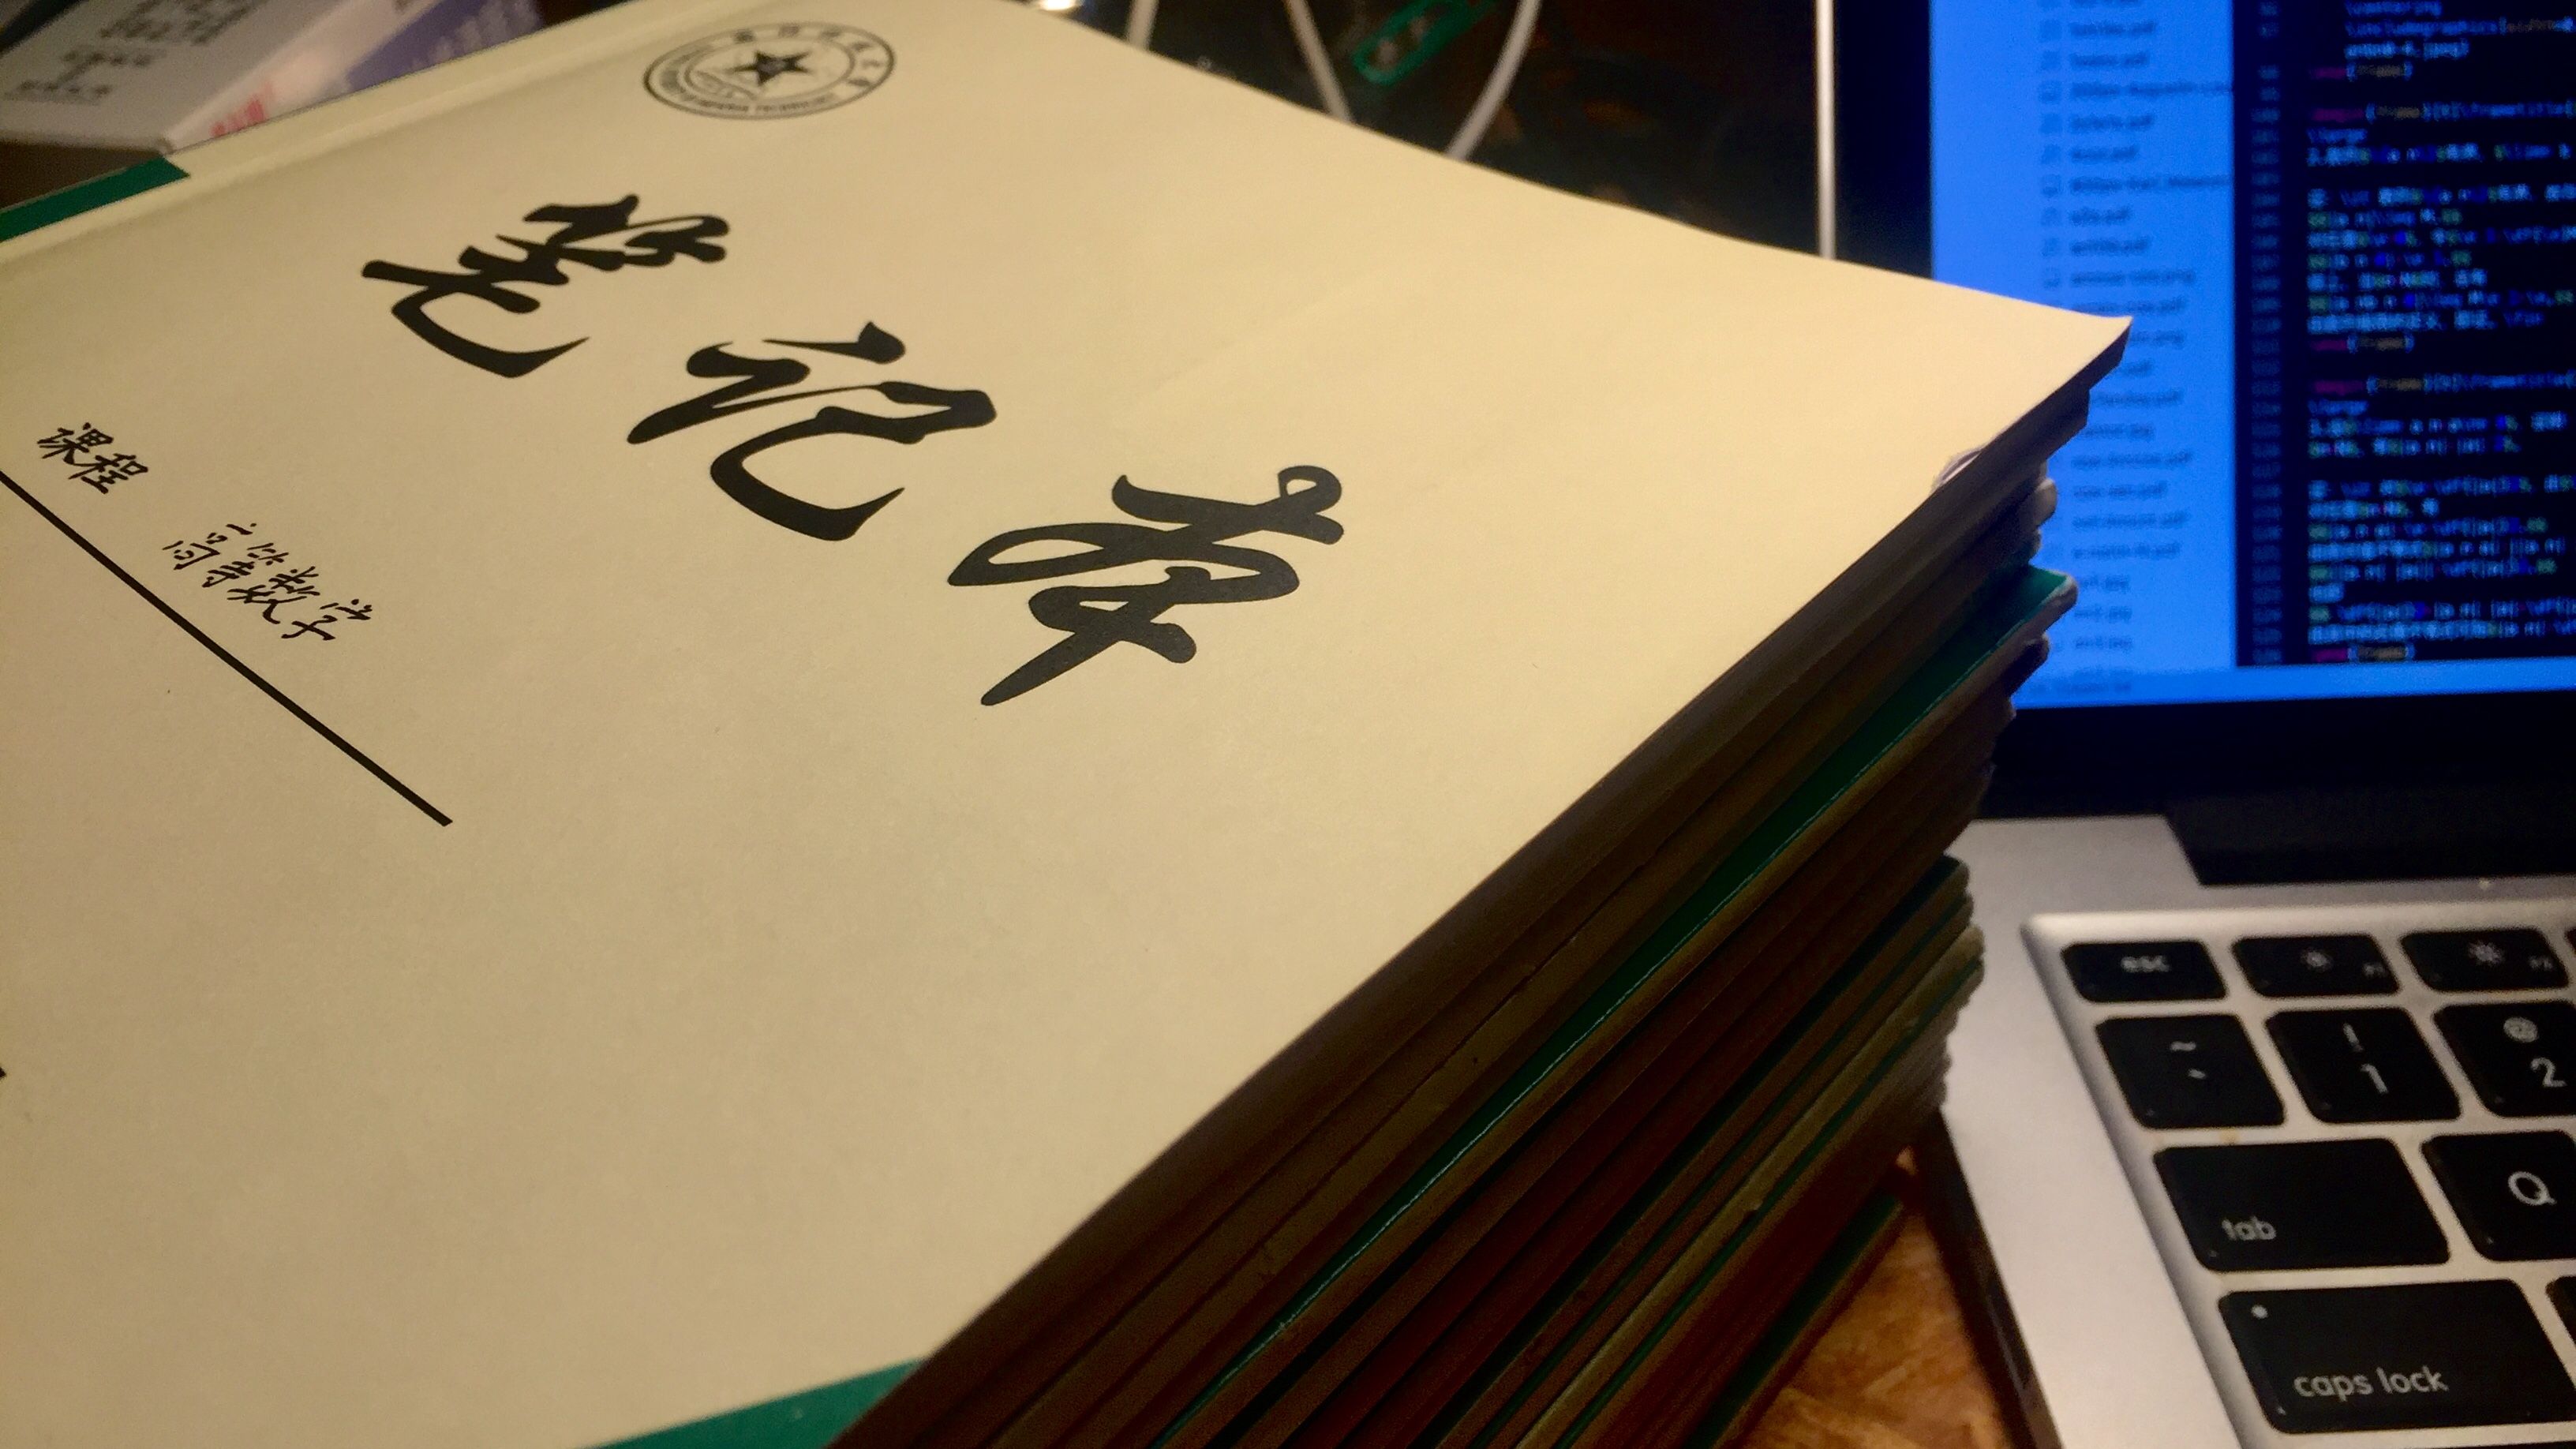
\includegraphics[width=0.9\textwidth]{./images/ch01/HWR/notebook.jpg}
\end{frame}

\end{document}